\documentclass[12pt,a4paper]{article}

\usepackage[a4paper,margin=1in]{geometry}
\usepackage[T1]{fontenc}
\usepackage[utf8]{inputenc}
\usepackage{lmodern}
\usepackage{amsmath,amssymb}
\usepackage{booktabs}
\usepackage{array}
\usepackage{float}
\usepackage{graphicx}
\usepackage{threeparttable}
\usepackage[authoryear]{natbib}
\usepackage{hyperref}
\usepackage{xcolor}

\hypersetup{
  colorlinks=true,
  linkcolor=blue!50!black,
  urlcolor=blue!50!black,
  citecolor=blue!50!black
}

\setlength{\parindent}{2em}
\setlength{\parskip}{0.5em}
\renewcommand{\arraystretch}{1.15}
\linespread{1.15}\selectfont

\title{The Exchange Rate and Japanese Tourist Arrivals to Taiwan:\\Evidence from Monthly Data, 2009--2019}
\author{Econometrics Final Project Report}
\date{\today}

\begin{document}

\maketitle

\begin{abstract}
This paper examines whether movements in the bilateral Taiwan--Japan exchange rate are associated with Japanese tourist arrivals to Taiwan. Using monthly data from October 2009 to December 2019, I estimate log-linear tourism demand models with Newey--West standard errors to account for serial correlation and heteroskedasticity in the residuals. The empirical specification includes 11 month dummies to capture seasonality, Japanese industrial production to proxy origin-country demand conditions, and Brent oil prices to proxy transportation costs. The baseline bivariate regression suggests a statistically significant negative relationship between the exchange rate and tourist arrivals. However, once seasonal effects, a linear time trend, Japanese industrial production, and oil prices are added, the exchange rate coefficient becomes small and statistically insignificant. A dynamic model with lagged tourist arrivals shows strong persistence in tourism flows, while additional robustness checks based on distributed lags and first differences also fail to produce stable evidence of a positive exchange-rate elasticity. Overall, the results suggest that the bilateral exchange rate alone is not a robust predictor of Japanese arrivals to Taiwan during the sample period.

\textbf{Keywords:} tourism demand, exchange rate, Taiwan, Japan, time-series regression
\end{abstract}

\section{Introduction}

Japan is one of Taiwan's most important inbound tourism markets, and changes in the bilateral exchange rate may affect how expensive Taiwan appears to Japanese travelers. When the yen strengthens against the New Taiwan dollar, Japanese tourists gain purchasing power in Taiwan, which could increase travel demand. This mechanism is standard in tourism economics because relative prices influence destination choice, trip timing, and on-site spending.

At the same time, exchange rates are not the only determinant of tourism flows. Tourism demand is also shaped by income conditions in the origin country, airfare and transport capacity, destination-specific marketing, seasonality, and broader macroeconomic shocks. If those factors are omitted, the exchange-rate coefficient may capture unrelated trends instead of a clean price effect. For that reason, a simple regression can be misleading even when the underlying economic intuition is plausible.

There is also a straightforward everyday intuition behind the control variables used in this paper. Japanese travelers do not decide on Taiwan trips only by looking at exchange-rate quotes. They also care about when holidays occur, whether low-cost carriers and regular airlines are operating enough seats, whether ticket prices are high because fuel is expensive, and whether Japan's domestic economy is strong enough to support discretionary travel. Golden Week, summer holidays, and year-end travel seasons can generate large predictable spikes in outbound tourism even if the exchange rate barely moves. Similarly, when oil prices rise, airlines may face cost pressure that eventually passes through to airfares. These practical considerations motivate the inclusion of 11 monthly dummies, Brent oil prices, and Japanese industrial production in the regression design.

This report studies whether the exchange rate remains relevant after these additional factors are taken into account. The empirical analysis uses monthly data from October 2009 to December 2019. The dependent variable is Japanese tourist arrivals to Taiwan. The main explanatory variable is the logarithm of the bilateral exchange rate, defined so that a higher value means stronger Japanese purchasing power in Taiwan. I complement the exchange-rate series with Japanese industrial production, Brent oil prices as a proxy for transportation costs, 11 monthly dummy variables, and a time trend.

The main result is straightforward. A simple bivariate model shows a significant negative association between the exchange rate and tourist arrivals, but that result is not robust. In the preferred specification with time and seasonal controls, the exchange-rate elasticity is small and statistically insignificant. This pattern suggests that secular tourism growth and strong seasonality are more important than short-run currency movements in explaining Japanese arrivals to Taiwan during this period.

\section{Literature Review}

The tourism-demand literature has long emphasized that tourist arrivals are shaped by income, relative prices, exchange rates, and destination-specific shocks. \citet{lim1997} reviews earlier international tourism-demand models and shows that empirical findings are highly sensitive to specification choices, omitted variables, and diagnostic testing. \citet{songli2008} extend this discussion and note that tourism forecasting and tourism-demand estimation are particularly sensitive to data frequency, seasonality, and structural shocks.

Several studies focus more directly on exchange rates and price competitiveness. \citet{webber2001} show that exchange-rate volatility can matter for long-run tourism demand, although the size and sign of the effect vary across destinations. \citet{seetaram2016} argue that the real exchange rate is often an imperfect proxy for tourism prices and show that the estimated price elasticity can change substantially when a more refined competitiveness index is used. This point is directly relevant here because the bilateral nominal exchange rate may not fully capture the travel cost faced by Japanese tourists visiting Taiwan. More recently, \citet{he2025} analyze international air transport and show that exchange-rate fluctuations can operate through both demand and supply channels. Their monthly route-level study finds that moderate exchange-rate fluctuations significantly affect passenger demand, while severe fluctuations can affect airfare through the supply side. Although their setting is airline routes linked to mainland China rather than tourism flows to Taiwan, the paper is useful because it highlights two ideas that matter for this project: exchange-rate effects may be nonlinear, and transport-cost channels should be modeled rather than ignored.

The literature also suggests that dynamic behavior matters. \citet{morley2009} emphasizes that tourism-demand models should treat dynamics carefully because travel flows often display persistence and delayed responses. In a more origin-specific setting, \citet{huiyuen1998} analyze Japanese tourist arrivals to British Columbia and highlight the importance of estimating demand at the source-market level rather than relying only on aggregate tourism totals. Following these insights, this paper models Japanese arrivals separately, includes seasonal controls, and compares static, dynamic, and first-difference specifications.

\section{Methodology}

The preferred empirical specification is a log-linear monthly tourism-demand model:

\begin{equation}
\ln(Tourist_t) = \beta_0 + \beta_1 \ln(FX_t) + \beta_2 \ln(JIPI_t) + \beta_3 \ln(Oil_t) + \beta_4 Trend_t + \beta_5 Crisis_t + \sum_{m=1}^{11} \delta_m Month_{m,t} + \varepsilon_t
\end{equation}

where $Tourist_t$ is monthly Japanese tourist arrivals to Taiwan, $FX_t$ is the bilateral exchange-rate measure, $JIPI_t$ is Japanese industrial production, $Oil_t$ is the Brent crude oil price, $Trend_t$ is a linear time trend, $Crisis_t$ is a dummy for major macroeconomic disruptions when such observations are available, and $Month_{m,t}$ are month fixed effects with December omitted as the reference month.

The coefficient of interest is $\beta_1$. Because both the dependent variable and the exchange-rate variable are in logarithms, $\beta_1$ is an elasticity. Holding other variables constant, a 1 percent increase in $FX_t$ is associated with approximately a $\beta_1$ percent change in tourist arrivals. Since the exchange-rate variable is defined so that a higher value means stronger Japanese purchasing power in Taiwan, the expected sign is positive. If the estimate is zero or insignificant, then exchange-rate movements may be less important than trend, seasonality, or other omitted travel determinants.

To examine dynamic persistence, I also estimate:

\begin{equation}
\ln(Tourist_t) = \alpha_0 + \alpha_1 \ln(Tourist_{t-1}) + \alpha_2 \ln(FX_t) + \alpha_3 \ln(JIPI_t) + \alpha_4 \ln(Oil_t) + \sum_{m=1}^{11} \lambda_m Month_{m,t} + u_t
\end{equation}

Equation (2) allows current tourism demand to depend on its own lag. This is useful because booking behavior, airline scheduling, and destination popularity may create persistence over time. In addition, the robustness section estimates a distributed-lag model for the exchange rate and a first-difference model to see whether the main result survives alternative treatments of trending behavior.

The main econometric concern is omitted-variable bias. Exchange rates may move alongside global financial conditions, transportation costs, or shifts in tourism demand that are not fully observed in the dataset. For that reason, the results should be interpreted as conditional associations rather than causal estimates.

It is also important to distinguish different types of black-swan events. The global financial crisis and the COVID-19 pandemic should not be pooled into a single shock category because they operate through different mechanisms. The financial crisis was primarily a macroeconomic demand shock that affected income, confidence, and discretionary spending, while the cross-border tourism market itself remained open. By contrast, the pandemic involved direct border closures, quarantine rules, and administrative restrictions that broke the normal price-demand mechanism altogether. Therefore, pandemic years should be excluded from the baseline tourism-demand sample, whereas the financial-crisis period, if present in the data, should be handled with a separate crisis dummy or a split-sample check rather than treated as equivalent to the pandemic.

As a practical extension, foreign-exchange forecasting models such as ARIMA, SARIMA, and SARIMAX can also be used to generate exchange-rate scenarios before the tourism-demand regression is estimated. Two public GitHub projects provided by the user illustrate this workflow. One project uses monthly FRED data for five currencies against the U.S. dollar and compares ARIMA, SARIMA, and SARIMAX models, with SARIMAX incorporating inflation, interest-rate, and trade-related exogenous variables for USD/INR forecasting \citep{rindhujatreesa_repo}. Another project demonstrates a simpler ARIMA-based forecasting exercise for the euro--U.S.-dollar rate \citep{shridhar_repo}. These repositories are not academic studies, so they are not used as empirical evidence in the literature review. However, they are useful implementation references for a future appendix in which the Taiwan--Japan exchange rate itself is forecasted and then fed into a tourism-demand scenario analysis.

\section{Data and Empirical Results}

\subsection{Data}

The sample consists of monthly observations from October 2009 to December 2019, yielding 123 observations. The unit of observation is a month. The tourism series comes from the Taiwan Tourism Administration's inbound visitors database, specifically the Japan inbound visitor counts. The exchange-rate series is based on the JPY/TWD currency page on Investing.com, which presents the Japanese yen to Taiwan dollar exchange rate and allows monthly observations to be tracked. Brent crude oil prices come from the FRED series POILBREUSDM, which is described as the global price of Brent crude in U.S. dollars per barrel, monthly and not seasonally adjusted, with the underlying source listed as the International Monetary Fund. Japanese industrial production comes from the FRED series JPNPRINTO01IXOBM, which is a monthly, not seasonally adjusted index for production volume in industry excluding construction, with 2015 = 100. The bilateral exchange-rate variable in the dataset is expressed so that a larger value represents stronger Japanese purchasing power in Taiwan. Japanese industrial production is used as a proxy for origin-country business conditions, and Brent crude oil prices proxy for broad transport-cost conditions.

Conceptually, the preferred pre-pandemic window for this project is 2008--2019 because it excludes the years in which border closures mechanically suppressed international travel. However, the Excel file provided for estimation begins in October 2009 rather than January 2008, so the actual regression sample is October 2009 to December 2019. This means the empirical exercise still separates the pandemic from the normal tourism period, but it can only capture the late stage of the global financial-crisis aftermath rather than the full 2008 crisis window. If earlier monthly data are later added, the same framework can be extended directly to a full 2008--2019 sample with a dedicated financial-crisis dummy.

\begin{table}[H]
\centering
\caption{Variable Definitions}
\label{tab:variables}
\begin{tabular}{p{3.0cm}p{7.1cm}p{3.3cm}p{1.5cm}}
\toprule
Variable & Definition & Source & Expected Sign \\
\midrule
$Tourist_t$ & Monthly Japanese tourist arrivals to Taiwan & Taiwan Tourism Administration & N/A \\
$\ln(FX_t)$ & Log of Taiwan dollars per Japanese yen; a higher value means a stronger yen in Taiwan & Central Bank of the Republic of China (Taiwan), author's construction & $+$ \\
$\ln(JIPI_t)$ & Log Japanese industrial production index & OECD & $+$ \\
$\ln(Oil_t)$ & Log Brent crude oil price & FRED / IMF & $-$ \\
$Month_{m,t}$ & Eleven month dummy variables; December is the omitted reference month & Author's construction & Varies \\
$Trend_t$ & Linear monthly trend & Author's construction & Ambiguous \\
$Crisis_t$ & Financial-crisis dummy when 2008 observations are available; conceptually distinct from pandemic exclusion & Author's construction & $-$ \\
\bottomrule
\end{tabular}
\end{table}

\begin{table}[H]
\centering
\caption{Summary Statistics}
\label{tab:summary}
\begin{tabular}{lccccc}
\toprule
Variable & Mean & SD & Min & Max & N \\
\midrule
Japanese tourist arrivals & 98896.886 & 31390.930 & 46249.000 & 177804.000 & 123 \\
Log tourist arrivals & 11.452 & 0.321 & 10.742 & 12.088 & 123 \\
Log exchange rate & -1.181 & 0.132 & -1.381 & -0.930 & 123 \\
Log Japanese industrial production & 4.615 & 0.053 & 4.451 & 4.750 & 123 \\
Log Brent oil price & 4.327 & 0.338 & 3.467 & 4.826 & 123 \\
\bottomrule
\end{tabular}
\begin{minipage}{0.9\textwidth}
\vspace{0.4em}\footnotesize Notes: The sample covers monthly observations from October 2009 to December 2019.
\end{minipage}
\end{table}

\begin{table}[H]
\centering
\caption{Correlation Matrix}
\label{tab:corr}
\begin{tabular}{lrrrr}
\toprule
Variable & (1) & (2) & (3) & (4) \\
\midrule
Log tourist arrivals & 1.000 & -0.596 & 0.261 & -0.421 \\
Log exchange rate & -0.596 & 1.000 & -0.058 & 0.598 \\
Log Japanese industrial production & 0.261 & -0.058 & 1.000 & -0.046 \\
Log Brent oil price & -0.421 & 0.598 & -0.046 & 1.000 \\
\bottomrule
\end{tabular}
\end{table}


Table \ref{tab:summary} shows that average monthly Japanese arrivals were about 98,897 during the sample period, with substantial variation across months. The exchange-rate series also varies meaningfully, although much less than tourist arrivals. Table \ref{tab:corr} reports simple correlations. The correlation between the exchange rate and tourist arrivals is negative in the raw data, which already suggests that a naive bivariate regression may not recover the structural relationship implied by tourism theory. By contrast, tourist arrivals are positively correlated with Japanese industrial production and negatively correlated with oil prices, although these simple correlations do not control for trend or seasonality.

Figure \ref{fig:index} plots both tourist arrivals and the exchange-rate index normalized to 100 in October 2009. The figure highlights an important feature of the data: tourist arrivals trend upward over time, while the exchange rate follows shorter-run swings. This difference in underlying time-series behavior helps explain why a simple bivariate regression can be misleading.

\begin{figure}[H]
\centering
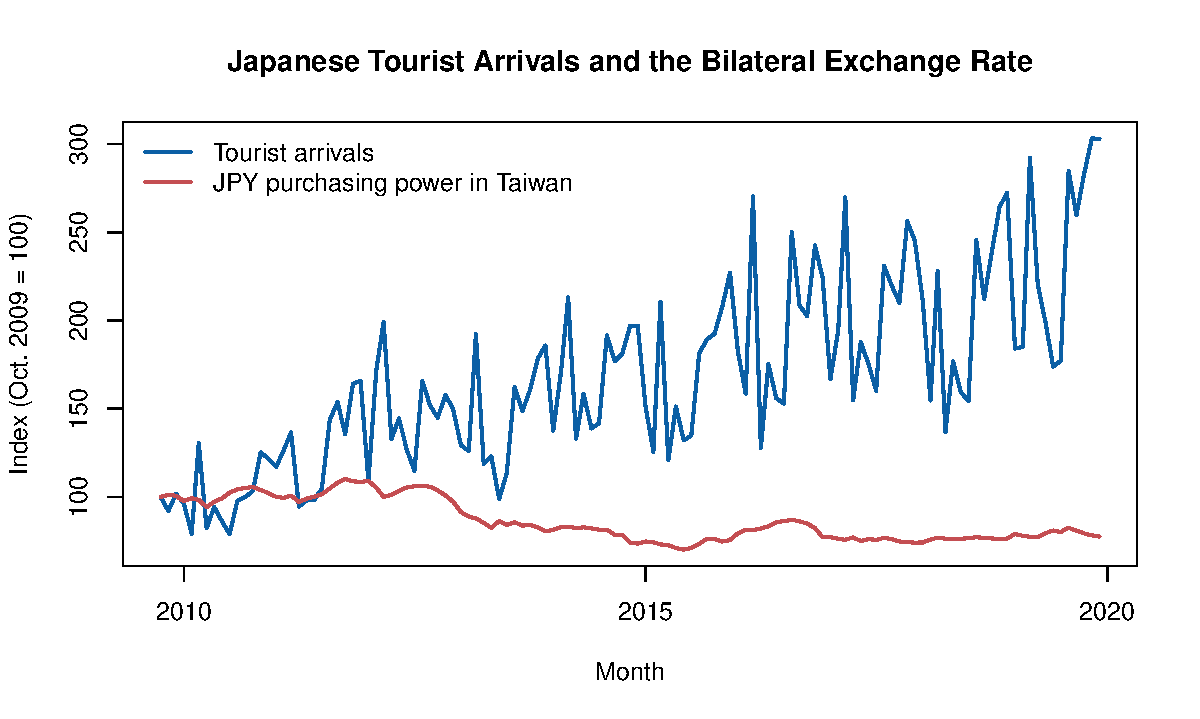
\includegraphics[width=0.88\textwidth]{output/tourism_fx_index.pdf}
\caption{Tourist Arrivals and the Exchange Rate Index}
\label{fig:index}
\end{figure}

\subsection{Empirical Results}

\begin{table}[H]
\centering
\caption{Baseline Regression Results}
\label{tab:mainreg}
\begin{threeparttable}
\begin{tabular}{lccc}
\toprule
 & (1) & (2) & (3) \\
Variables & Bivariate & Full Model & Dynamic Model \\
\midrule
Log exchange rate & -1.454*** & 0.119 & -0.264*** \\
 & (0.407) & (0.215) & (0.084) \\
Log Japanese industrial production &  & 0.260 & 0.768*** \\
 &  & (0.511) & (0.270) \\
Log Brent oil price &  & 0.073 & 0.006 \\
 &  & (0.086) & (0.036) \\
Time trend &  & 0.008*** &  \\
 &  & (0.001) &  \\
Lagged log tourist arrivals &  &  & 0.816*** \\
 &  &  & (0.053) \\
\midrule
Month fixed effects & No & Yes & Yes \\
Observations & 123 & 123 & 122 \\
$R^2$ & 0.356 & 0.891 & 0.895 \\
\bottomrule
\end{tabular}
\begin{tablenotes}[flushleft]
\footnotesize \item Notes: The dependent variable is the logarithm of monthly Japanese tourist arrivals to Taiwan. Newey--West standard errors with 12 lags are reported in parentheses. December is the omitted month in models with seasonal controls. *** $p<0.01$, ** $p<0.05$, * $p<0.10$.
\end{tablenotes}
\end{threeparttable}
\end{table}

\begin{table}[H]
\centering
\caption{Detailed OLS Output for the Full Model}
\label{tab:statafull}
\begin{minipage}{0.48\textwidth}
\centering
\begin{tabular}{lrrrr}
\toprule
Source & SS & df & MS & \\
\midrule
Model & 11.1855 & 15 & 0.7457 & \\
Residual & 1.3738 & 107 & 0.0128 & \\
Total & 12.5593 & 122 & 0.1029 & \\
\bottomrule
\end{tabular}
\end{minipage}
\hfill
\begin{minipage}{0.44\textwidth}
\centering
\begin{tabular}{lr}
\toprule
Statistic & Value \\
\midrule
Number of obs & 123 \\
$F(15,107)$ & 58.08 \\
Prob $>$ $F$ & 0.0000 \\
$R^2$ & 0.8906 \\
Adj. $R^2$ & 0.8753 \\
Root MSE & 0.1133 \\
\bottomrule
\end{tabular}
\end{minipage}
\vspace{0.8em}
\begin{tabular}{lrrrrr}
\toprule
Variable & Coef. & Std. Err. & $t$ & $P>|t|$ & 95\% CI \\
\midrule
Constant & 9.7729 & 1.6199 & 6.03 & 0.0000 & [6.5616, 12.9841] \\
Log exchange rate & 0.1189 & 0.1402 & 0.85 & 0.3983 & [-0.1591, 0.3969] \\
Log Japanese industrial production & 0.2601 & 0.3447 & 0.75 & 0.4521 & [-0.4232, 0.9434] \\
Log Brent oil price & 0.0734 & 0.0391 & 1.87 & 0.0637 & [-0.0042, 0.1510] \\
Time trend & 0.0078 & 0.0005 & 15.15 & 0.0000 & [0.0068, 0.0089] \\
\bottomrule
\end{tabular}
\begin{minipage}{0.95\textwidth}
\vspace{0.4em}\footnotesize Notes: This table follows the conventional OLS output style used by Stata. Coefficient inference here is based on classical OLS standard errors. The main comparison tables in the paper additionally report Newey--West standard errors.
\end{minipage}
\end{table}

\begin{table}[H]
\centering
\caption{Detailed OLS Output for the Dynamic Model}
\label{tab:statadyn}
\begin{minipage}{0.48\textwidth}
\centering
\begin{tabular}{lrrrr}
\toprule
Source & SS & df & MS & \\
\midrule
Model & 11.0369 & 15 & 0.7358 & \\
Residual & 1.2974 & 106 & 0.0122 & \\
Total & 12.3343 & 121 & 0.1019 & \\
\bottomrule
\end{tabular}
\end{minipage}
\hfill
\begin{minipage}{0.44\textwidth}
\centering
\begin{tabular}{lr}
\toprule
Statistic & Value \\
\midrule
Number of obs & 122 \\
$F(15,106)$ & 60.12 \\
Prob $>$ $F$ & 0.0000 \\
$R^2$ & 0.8948 \\
Adj. $R^2$ & 0.8799 \\
Root MSE & 0.1106 \\
\bottomrule
\end{tabular}
\end{minipage}
\vspace{0.8em}
\begin{tabular}{lrrrrr}
\toprule
Variable & Coef. & Std. Err. & $t$ & $P>|t|$ & 95\% CI \\
\midrule
Constant & -1.7554 & 1.6191 & -1.08 & 0.2807 & [-4.9656, 1.4547] \\
Lagged log tourist arrivals & 0.8159 & 0.0528 & 15.46 & 0.0000 & [0.7112, 0.9205] \\
Log exchange rate & -0.2645 & 0.1201 & -2.20 & 0.0298 & [-0.5025, -0.0264] \\
Log Japanese industrial production & 0.7684 & 0.3338 & 2.30 & 0.0233 & [0.1067, 1.4302] \\
Log Brent oil price & 0.0056 & 0.0378 & 0.15 & 0.8828 & [-0.0693, 0.0804] \\
\bottomrule
\end{tabular}
\begin{minipage}{0.95\textwidth}
\vspace{0.4em}\footnotesize Notes: This table follows the conventional OLS output style used by Stata. Coefficient inference here is based on classical OLS standard errors. The main comparison tables in the paper additionally report Newey--West standard errors.
\end{minipage}
\end{table}


Table \ref{tab:mainreg} reports the main regression results. Column (1) estimates a simple bivariate regression and produces a coefficient of $-1.454$ on the log exchange rate, significant at the 1 percent level. Interpreted mechanically, this would imply that a 1 percent increase in Japanese purchasing power in Taiwan is associated with a 1.454 percent \emph{decrease} in Japanese arrivals. This sign is counterintuitive and likely reflects omitted factors rather than a true tourism-price effect.

Column (2) adds Japanese industrial production, oil prices, a linear time trend, and 11 monthly dummy variables. Once these controls are included, the exchange-rate coefficient becomes $0.119$ and is no longer statistically significant. According to Equation (1), holding other variables constant, a 1 percent increase in the exchange-rate variable is associated with only a 0.119 percent increase in tourist arrivals, and the estimate is too imprecise to distinguish from zero. The strongest predictor in this specification is the time trend, while the joint month-dummy test later shows that seasonal structure is also essential. This suggests that the sample contains substantial secular growth in Japanese tourism to Taiwan that would otherwise be absorbed by the exchange-rate term.

Column (3) introduces lagged log tourist arrivals. The lagged dependent variable is large and highly significant, with a coefficient of $0.816$, indicating strong persistence in tourism flows. In this dynamic specification, the contemporaneous exchange-rate coefficient turns negative again and is statistically significant. I interpret this result cautiously. Once persistence is modeled directly, short-run deviations in arrivals may reflect timing adjustments, backlog effects, or model sensitivity rather than a stable structural elasticity.

The two detailed OLS tables provide the same result in a format closer to standard software output. In Table \ref{tab:statafull}, the full model has an $R^2$ of 0.891, an adjusted $R^2$ of 0.875, and an overall $F$-statistic of 58.08. The time trend is highly significant, while the exchange-rate coefficient is not. Table \ref{tab:statadyn} shows that the dynamic model raises the explanatory power slightly and confirms that the lagged dependent variable dominates short-run variation in arrivals. These detailed tables make it clear that the main empirical issue is not low fit, but unstable interpretation of the exchange-rate coefficient across specifications.

\section{Robustness Check and Additional Tests}

\begin{table}[H]
\centering
\caption{Robustness Checks}
\label{tab:robust}
\begin{threeparttable}
\begin{tabular}{lccc}
\toprule
 & (1) & (2) & (3) \\
Variables & Full Model & Distributed Lag & First Difference \\
\midrule
Log exchange rate & 0.119 & -0.481 &  \\
 & (0.215) & (0.433) &  \\
Lagged log exchange rate ($t-1$) &  & 0.261 &  \\
 &  & (0.506) &  \\
Lagged log exchange rate ($t-2$) &  & 0.406 &  \\
 &  & (0.564) &  \\
Sum of exchange rate terms &  & 0.186 &  \\
 &  & (0.229) &  \\
Change in log exchange rate &  &  & -0.075 \\
 &  &  & (0.638) \\
Log Japanese industrial production & 0.260 & 0.285 &  \\
 & (0.511) & (0.549) &  \\
Change in log Japanese industrial production &  &  & 1.036*** \\
 &  &  & (0.203) \\
Log Brent oil price & 0.073 & 0.035 &  \\
 & (0.086) & (0.090) &  \\
Change in log Brent oil price &  &  & -0.089 \\
 &  &  & (0.199) \\
\midrule
Month fixed effects & Yes & Yes & No \\
Time trend & Yes & Yes & No \\
Observations & 123 & 121 & 122 \\
$R^2$ & 0.891 & 0.895 & 0.100 \\
\bottomrule
\end{tabular}
\begin{tablenotes}[flushleft]
\footnotesize \item Notes: Column (2) adds one- and two-month lags of the exchange rate. Column (3) estimates the model in first differences to remove level trends. Newey--West standard errors with 12 lags are reported in parentheses. *** $p<0.01$, ** $p<0.05$, * $p<0.10$.
\end{tablenotes}
\end{threeparttable}
\end{table}

\begin{table}[H]
\centering
\caption{Hypothesis Tests}
\label{tab:hypothesis}
\begin{tabular}{p{6.1cm}rrr}
\toprule
Null hypothesis & Test statistic & $p$-value & Decision at 5\% \\
\midrule
$H_0$: Exchange-rate elasticity in the full model equals zero & 0.552 & 0.5821 & Fail to reject \\
$H_0$: Month effects are jointly zero & 20.563 & 0.0000 & Reject \\
$H_0$: Exchange rate and all 11 month dummies are jointly zero & 19.055 & 0.0000 & Reject \\
$H_0$: Japanese industrial production and oil price are jointly zero & 2.084 & 0.1294 & Fail to reject \\
$H_0$: Oil price coefficient in the full model equals zero & 0.849 & 0.3976 & Fail to reject at 5\% \\
$H_0$: Lagged exchange-rate terms are jointly zero & 1.011 & 0.3673 & Fail to reject \\
$H_0$: Lagged tourist arrivals have no explanatory power & 238.968 & 0.0000 & Reject \\
$H_0$: Sum of exchange-rate coefficients in the distributed-lag model equals zero & 0.664 & 0.4171 & Fail to reject \\
\bottomrule
\end{tabular}
\end{table}

\begin{table}[H]
\centering
\caption{Regression Diagnostic Tests}
\label{tab:diagnostics}
\begin{tabular}{lrrrr}
\toprule
Model & Durbin--Watson & Breusch--Godfrey(12) & Breusch--Pagan & RESET \\
\midrule
Bivariate & 0.933 (0.0000) & 67.965 (0.0000) & 0.012 (0.9119) & 16.871 (0.0000) \\
Full model & 1.061 (0.0000) & 42.577 (0.0000) & 34.154 (0.0032) & 0.813 (0.4464) \\
Dynamic & 2.668 (0.9995) & 26.813 (0.0082) & 36.102 (0.0017) & 0.539 (0.5848) \\
Distributed lag & 1.073 (0.0000) & 45.930 (0.0000) & 42.927 (0.0005) & 0.688 (0.5049) \\
\bottomrule
\end{tabular}
\begin{minipage}{0.95\textwidth}
\vspace{0.4em}\footnotesize Notes: Each cell reports the test statistic followed by its $p$-value in parentheses. The null hypotheses are no first-order residual autocorrelation for Durbin--Watson, no higher-order serial correlation for Breusch--Godfrey, homoskedasticity for Breusch--Pagan, and correct functional form for RESET.
\end{minipage}
\end{table}

\begin{table}[H]
\centering
\caption{ADF-Style Unit-Root and Spurious-Regression Checks}
\label{tab:adf}
\begin{tabular}{lrrl}
\toprule
Series & Level statistic & First-difference statistic & Approximate conclusion \\
\midrule
Log tourist arrivals & -6.025 & -13.513 & Level-stationary at 5\% \\
Log exchange rate & -1.831 & -6.119 & Likely I(1) \\
Log Japanese industrial production & -10.496 & -20.373 & Level-stationary at 5\% \\
Log Brent oil price & -2.066 & -7.070 & Likely I(1) \\
\midrule
Residual from bivariate regression & -3.748 & -- & Stationary residual if statistic $<$ -2.89 \\
Residual from full regression & -4.331 & -- & Stationary residual if statistic $<$ -2.89 \\
\bottomrule
\end{tabular}
\begin{minipage}{0.95\textwidth}
\vspace{0.4em}\footnotesize Notes: These are manual ADF-style regressions with one lag of the dependent difference. For level tests, the regression includes an intercept and linear trend; for first differences and residuals, it includes an intercept only. As a rule of thumb, a value below about $-3.43$ in levels with trend or below about $-2.89$ in differences suggests rejecting a unit root at the 5\% level. This table is used to screen for potential spurious regression concerns rather than to replace a full unit-root package.
\end{minipage}
\end{table}


Table \ref{tab:robust} evaluates whether the main conclusion changes under alternative specifications. Column (2) adds one- and two-month lags of the exchange rate. None of the individual exchange-rate terms is statistically significant, and the cumulative coefficient is $0.186$, which is also insignificant. This means there is no evidence in the sample that exchange-rate effects simply appear with a short delay.

Column (3) estimates the model in first differences. This approach removes level trends and focuses on month-to-month changes. The coefficient on the change in the exchange rate is $-0.075$ with a very large standard error, again providing no evidence of a stable exchange-rate effect. By contrast, changes in Japanese industrial production remain positive and significant in the differenced model, suggesting that short-run movements in Japanese macroeconomic conditions are more informative for tourism fluctuations than the bilateral exchange rate alone.

\subsection{Joint Hypothesis Tests}

Table \ref{tab:hypothesis} reports a broader set of targeted hypothesis tests. First, the null hypothesis that the exchange-rate elasticity in the full model equals zero cannot be rejected. Second, the month dummies are jointly significant, which confirms that seasonality is a central feature of the data and cannot be ignored. Third, the exchange rate together with the full set of month dummies is jointly significant, which implies that seasonal structure and price-related conditions matter in combination even though the exchange rate alone is weak in the preferred specification. Fourth, Japanese industrial production and oil prices are not jointly significant at the 5 percent level in the full specification, although industrial production becomes more important once the model is estimated in first differences. Fifth, oil prices by themselves are only marginally significant in the conventional OLS table and do not survive the more conservative Newey--West inference standard. Sixth, the lagged exchange-rate terms are not jointly significant in the distributed-lag model. Finally, the lagged dependent variable in the dynamic model is overwhelmingly significant, which supports the view that tourism flows are persistent over time. These tests reinforce the view that the exchange rate is not the main driver of Japanese arrivals once richer controls are introduced.

\subsection{Residual Diagnostics}

Table \ref{tab:diagnostics} examines whether the regressions satisfy common time-series regression assumptions. The bivariate, full, and distributed-lag models all show very strong evidence of serial correlation according to both the Durbin--Watson and Breusch--Godfrey tests. The full, dynamic, and distributed-lag models also reject homoskedasticity under the Breusch--Pagan test, which justifies the use of Newey--West standard errors in the main regression tables. By contrast, the RESET test rejects the bivariate specification but does not reject the richer models, suggesting that the more complete specifications are better aligned with the underlying functional form. In short, the raw OLS model is not reliable for inference without additional correction.

\subsection{Checking for Spurious Regression}

One of the user's main concerns is whether the regressions are ``fake'' or spurious. Table \ref{tab:adf} addresses this issue using ADF-style unit-root checks. The tourism series and Japanese industrial production appear stationary in levels once a trend is included, while the exchange-rate and oil-price series look more like $I(1)$ processes because the level statistic is weak but the first-difference statistic is strongly negative. This means the regression mixes variables with different time-series properties, which is exactly the type of environment in which spurious inference can arise if the model is not diagnosed carefully.

The residual checks provide an additional screen. The residuals from both the bivariate regression and the full model are sufficiently negative under the ADF-style residual regression, which weakens the claim that the estimated relationships are purely spurious in the Engle--Granger sense. However, this does not completely remove concern because serial correlation and heteroskedasticity remain strong, and the sign of the exchange-rate coefficient changes substantially across specifications. For that reason, the safest conclusion is not that the model proves no exchange-rate effect exists, but that the available monthly data do not deliver a stable and robust exchange-rate elasticity under several reasonable econometric tests.

Taken together, the robustness checks reinforce the main message of the paper. The exchange rate does not emerge as a robust determinant of Japanese arrivals once the model accounts for seasonality, trends, persistence, differencing, and diagnostic testing. The most defensible interpretation is that the bilateral exchange rate may matter at the margin, but its influence is dominated by broader demand conditions and long-run tourism trends during 2009--2019.

\section{Conclusion}

This paper studies whether the Taiwan--Japan exchange rate is associated with Japanese tourist arrivals to Taiwan using monthly data from October 2009 to December 2019. The empirical strategy estimates log-linear time-series regressions with Newey--West standard errors and compares a simple bivariate model with richer specifications that add macro controls, seasonality through 11 monthly dummies, oil prices as a transportation-cost proxy, dynamics, and alternative transformations.

The results do not support a robust positive exchange-rate elasticity. Although the bivariate regression produces a statistically significant coefficient, the sign is counterintuitive and disappears once trend and seasonal controls are added. The preferred full model implies a small and statistically insignificant elasticity, while distributed-lag and first-difference models lead to the same conclusion. The data therefore suggest that Japanese arrivals to Taiwan were driven more strongly by persistent tourism growth, seasonal patterns, and origin-country macro conditions than by bilateral currency movements alone.

This report still has limitations. First, the dataset does not include direct measures of airfare, flight capacity, or Taiwan-specific tourism promotion, all of which could improve the specification. Second, the exchange-rate measure is nominal rather than real, so it does not fully account for relative inflation. Third, although the conceptual pre-pandemic design is 2008--2019, the supplied file starts in late 2009, so the full financial-crisis episode cannot yet be modeled directly with a separate dummy. Future research could extend the model with real exchange rates, airline supply variables, a complete 2008--2019 monthly series, or purpose-specific tourism categories to determine whether exchange-rate sensitivity is stronger for some traveler segments than for total leisure arrivals.

\begin{thebibliography}{99}

\bibitem[Central Bank of the Republic of China (Taiwan)(2026)]{cbc2026}
Central Bank of the Republic of China (Taiwan) (2026). Monthly exchange rate statistics. Official online database, accessed May 25, 2026.

\bibitem[Federal Reserve Bank of St. Louis(2026)]{fred2026}
Federal Reserve Bank of St. Louis (2026). Global price of Brent Crude [POILBREUSDM]. Official online database, accessed May 25, 2026.

\bibitem[He et~al.(2025)]{he2025}
He, Y., W. Ma, K. Fan, H. Li, and K. Wang (2025). The impacts of exchange rate fluctuations on the international air transport. Transportation Research Part A: Policy and Practice 198, 104523.

\bibitem[Hui and Yuen(1998)]{huiyuen1998}
Hui, T.-K. and C.-C. Yuen (1998). An econometric study on Japanese tourist arrivals in British Columbia and its implications. The Service Industries Journal 18(4), 38--50.

\bibitem[Lim(1997)]{lim1997}
Lim, C. (1997). An econometric classification and review of international tourism demand models. Tourism Economics 3(1), 69--81.

\bibitem[Morley(2009)]{morley2009}
Morley, C. L. (2009). Dynamics in the specification of tourism demand models. Tourism Economics 15(1), 23--39.

\bibitem[OECD(2026)]{oecd2026}
OECD (2026). Industrial production. Official online database, accessed May 25, 2026.

\bibitem[Rindhujatreesa(n.d.)]{rindhujatreesa_repo}
Rindhujatreesa (n.d.). Foreign-exchange-rate-time-series-forecasting. GitHub repository, accessed May 25, 2026.

\bibitem[Seetaram et~al.(2016)]{seetaram2016}
Seetaram, N., P. Forsyth, and L. Dwyer (2016). Measuring price elasticities of demand for outbound tourism using competitiveness indices. Annals of Tourism Research 56, 65--79.

\bibitem[Shridhar1504(n.d.)]{shridhar_repo}
Shridhar1504 (n.d.). Foreign-Exchange-Rate-Time-series-Datascience-Project. GitHub repository, accessed May 25, 2026.

\bibitem[Song and Li(2008)]{songli2008}
Song, H. and G. Li (2008). Tourism demand modelling and forecasting---A review of recent research. Tourism Management 29(2), 203--220.

\bibitem[Tourism Administration, MOTC(2026)]{tta2026}
Tourism Administration, Ministry of Transportation and Communications (2026). Tourism Statistics Database. Official online database, accessed May 25, 2026.

\bibitem[Webber(2001)]{webber2001}
Webber, A. G. (2001). Exchange rate volatility and cointegration in tourism demand. Journal of Travel Research 39(4), 398--405.

\end{thebibliography}

\end{document}
